\toolname is a post-synthesis refinement layer for LLM-generated vulnerability detectors.  Given a draft CSA checker or CodeQL query produced by an upstream generator, the patch that motivated the synthesis, and the corresponding source tree and validation scope, \toolname refines the detector to encode missing semantic predicates while preserving the vulnerable-side trigger.

% \subsection{Overview}

\begin{figure*}[t]
  \centering
  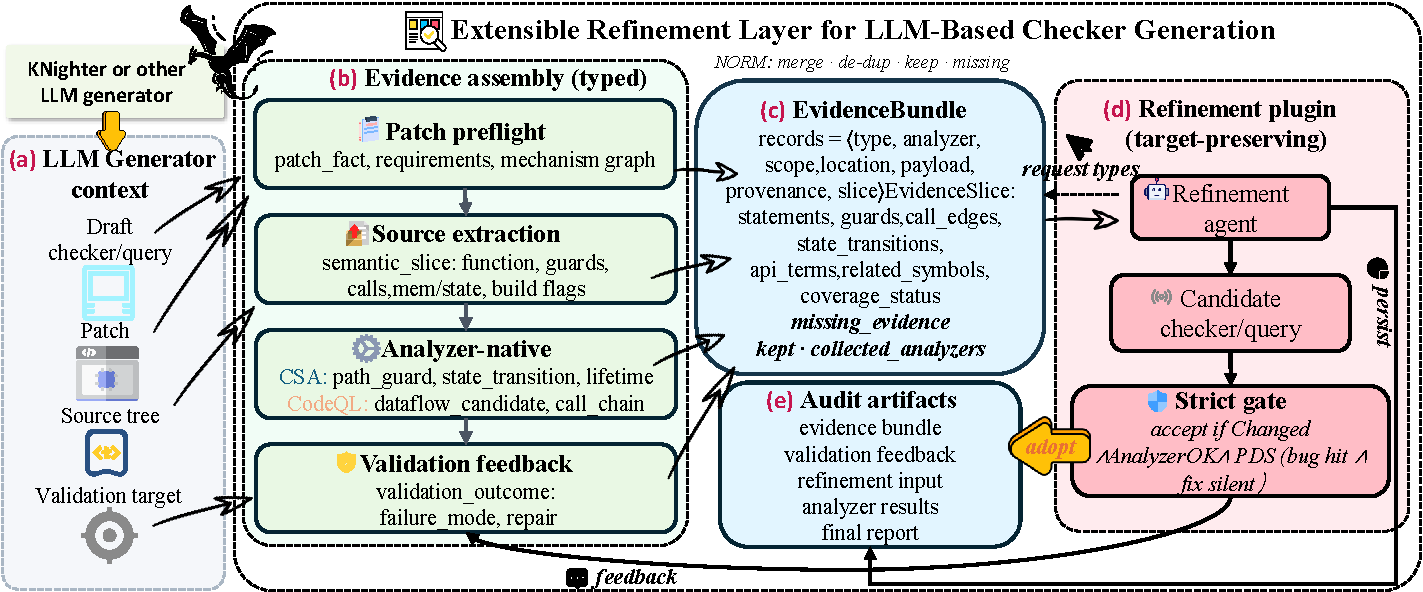
\includegraphics[width=\textwidth]{figures/fig-architecture.pdf}
  \Description{Workflow from a generated checker and patch through evidence collection, a typed provenance-labelled bundle, checker editing, paired validation, and audit artifacts.}
  \caption{\textbf{\toolname architecture.}
  (a)~An LLM generator produces a draft detector from the patch.
  (b)~A rule-guided patch preflight plans evidence requirements and four collectors gather corresponding facts; the figure's ``analyzer-native'' collector label does not mean every emitted record has internal provenance.
  (c)~Facts are normalized into a typed \texttt{EvidenceBundle} with seven persisted record types.
  (d)~The refinement agent edits the detector using role-specific views. A strict gate accepts only candidates that preserve the vulnerable-side trigger while silencing the fixed side. Rejected candidates feed back into the bundle (dashed arrow).
  (e)~Adopted candidates, evidence bundles, and validation logs are persisted as audit artifacts for reproducibility.}
  \label{fig:approach-architecture}
\end{figure*}

Figure~\ref{fig:approach-architecture} shows five stages.
\textbf{(a)~Generator context.}  \toolname receives a draft detector from an upstream LLM generator (e.g., KNighter), together with the patch, source tree, and validation target.  It treats the generator as a black box: any synthesized detector is an artifact to be refined, not regenerated.
\textbf{(b)~Evidence assembly.}  Rule-guided patch preflight infers a likely mechanism from patch facts and available analysis metadata, then prioritizes evidence requirements.  Four collectors (patch preflight, source extraction, analyzer representations or outputs from CSA/CodeQL, and validation feedback) gather evidence (Section~\ref{sec:adaptive-selection}).
\textbf{(c)~Evidence bundle.}  All facts are normalized into a typed \texttt{EvidenceBundle} with seven persisted record types, giving the refinement agent structured edit targets rather than raw analyzer dumps (Sections~\ref{sec:evidence-roles} and~\ref{sec:evidence-schema}).
\textbf{(d)~Target-preserving refinement.}  The refinement agent edits the detector using role-specific evidence views from the bundle.  A strict gate accepts a candidate only when it preserves the vulnerable-side trigger and eliminates fixed-side warnings.  Rejected candidates re-enter the bundle as feedback for the next iteration (Section~\ref{sec:refinement}).
\textbf{(e)~Audit artifacts.}  Each run persists the starting and candidate detector, evidence bundle, prompt/response trace, validation logs, and final report.  The verifier recomputes raw-output hashes, checks the recorded Clang interface/schema and patch file/function binding for every internal record, recounts provenance classes, and then checks the compiled candidate against paired vulnerable/fixed logs.  It does not infer evidence origin from an LLM explanation or rerun a model to reproduce a deterministic count.

\begin{algorithm}[t]
\footnotesize
\caption{Target-Preserving Evidence-Guided Refinement}
\label{alg:evidence-guided-refinement}
\begin{algorithmic}[1]
\Require detector $D$, patch $P$, source $S$, scope $V$, backends $A$, budget $K$
\Ensure refined detector $D^*$ and audit report
\State $R_0 \gets \Call{Validate}{D,P,V}$
\State $E_p,E_s \gets \Call{Preflight}{P},\ \Call{ExtractSource}{P,S,D}$
\State $E_a \gets \bigcup_{a\in A}\Call{CollectNative}{a,D,P,S}$ \quad $E_v \gets \Call{Feedback}{R_0}$
\State $B \gets \Call{NormalizeMerge}{E_p,E_s,E_a,E_v}$
\If{$\Call{PDS}{D,P,V}$}
  \State \Return $\Call{Audit}{D,B}$
\EndIf
\State $D^* \gets D$
\For{$i=1$ to $K$}
  \State $V_i \gets \Call{AgentSelectView}{B}$ \quad $C_i \gets \Call{AgentEdit}{D^*,P,V_i}$
  \State $R_i \gets \Call{Validate}{C_i,P,V}$
  \If{$\Call{Changed}{C_i,D^*} \land \Call{AnalyzerOK}{R_i} \land \Call{PDS}{C_i,P,V}$}
    \State $D^* \gets C_i$ \quad \textbf{break}
  \Else
    \State $E_i \gets \Call{Feedback}{R_i}$ \quad $B \gets \Call{Merge}{B,E_i}$
  \EndIf
\EndFor
\State \Return $\Call{Audit}{D^*,B}$
\end{algorithmic}
\end{algorithm}

\subsection{Adaptive Evidence Selection}
\label{sec:adaptive-selection}

The central design choice in evidence assembly~(Figure~\ref{fig:approach-architecture}b) is \emph{what to collect and expose}.  Analyzer outputs can be large and heterogeneous; passing them wholesale to the editor obscures patch-relevant relations.  The preflight planner represents candidate requirements by role and priority, while source/function scope and bounded views limit what the editor sees.  In the strict CSA comparison, collection is precomputed and the visible view is frozen, so its result does not measure demand-driven routing.

\textbf{Rule-guided preflight and role requests.}
The implementation has no separately trained or prompted patch-mechanism classifier.  \texttt{PatchFacts\allowbreak Extractor} parses the patch and metadata for affected functions, added guards, risky calls, and type widenings.  \texttt{Evidence\allowbreak Planner} takes a primary pattern from analysis metadata when available or infers it from those facts, then assigns fixed priorities to requirements: patch anchoring is 100, lifetime/state requirements for double-free or use-after-free are 92/89, and a guard for null or bounds cases is 90.  It sorts by descending priority with evidence type as a tie-breaker and retains at most eight planned requirements in the default configuration.  Table~\ref{tab:evidence-routing} summarizes mechanism-to-role examples; it is not a classifier confusion matrix or a promise that every role is analyzer-internal.  The normalizer does not learn or re-rank facts.  In the general workflow the editor may request evidence types, with duplicate and request-count limits.
For the strict provenance-audited CSA comparison, patch-scoped records are precomputed.  The treatment preloads up to the first four distinct strictly internal record types in persisted order and disables additional requests; its no-internal counterpart sees no internal records but retains patch, source, and feedback context.  This deterministic exposure policy is a limitation, not an adaptive classifier.  The matched result tests the frozen native-evidence view, \emph{not} a routing policy's accuracy or benefit.

\begin{table}[t]
\footnotesize
\centering
\setlength{\tabcolsep}{3pt}
\caption{Rule-guided evidence requirements by patch mechanism (representative); names are persisted record types, not gold labels or measured classifier outputs.}
\label{tab:evidence-routing}
\begin{tabular}{@{}p{0.32\columnwidth}p{0.40\columnwidth}p{0.18\columnwidth}@{}}
\toprule
\textbf{Patch mechanism} & \textbf{Possible record types} & \textbf{Backend} \\
\midrule
Cleanup edge / double free & \texttt{allocation\_lifecycle}, \texttt{state\_transition}, \texttt{path\_guard} & CSA \\
Bounds widening / overflow & \texttt{semantic\_slice}, \texttt{dataflow\_candidate}, \texttt{state\_transition} & CSA/CodeQL \\
Initialization / null deref & \texttt{state\_transition}, \texttt{path\_guard} & CSA \\
Use-after-free / escape & \texttt{allocation\_lifecycle}, \texttt{call\_chain} & CSA/CodeQL \\
API misuse / missing check & \texttt{semantic\_slice}, \texttt{call\_chain} & CodeQL \\
\bottomrule
\end{tabular}
\end{table}

\subsection{Evidence Sources and Roles}
\label{sec:evidence-roles}

Given the patch scope and any planned requirements, four collectors execute in sequence (Figure~\ref{fig:approach-architecture}b, top to bottom):

\textbf{Patch preflight} identifies changed files, hunks, and statements, and produces a mechanism graph that links the edited code to likely bug patterns.  This supplies the structural skeleton: \emph{what changed} and \emph{where}.

\textbf{Source extraction} resolves patch files and records bounded contexts around the changed code, including enclosing functions, branch guards, callee signatures, memory/state operations, and build flags.  This provides local semantic context without dumping repository-scale source.

\textbf{Analyzer evidence} is classified by its actual origin, not by the collector's name.  We call a record \emph{analyzer-internal} only if its payload is derived from a backend-produced intermediate representation, identifies the interface and raw output, and is bound to a source revision, file, and function.  In the measured CSA cohort the interface is Clang 18's \texttt{debug.DumpCFG} and \texttt{debug.DumpCallGraph}; the persisted UTF-8 dump is parsed into schema \texttt{semweaver.csa\_cfg\_snapshot.v1}, with a raw-output SHA-256 and source-scope binding.  These dumps provide CFG branches and value bindings and call edges.  They do \emph{not} themselves prove a path-feasible lifetime or ownership transition.  Analyzer diagnostics and alert counts are \emph{analyzer output}, not internal state.  Patch diffs, source windows, and compile-database-assisted source extraction are \emph{source-derived} fallbacks even when a CSA or CodeQL collector emits them.  A live CodeQL database query could meet the internal-evidence definition if its query, database revision, and tuples were retained; we do not attribute source-window-derived CodeQL facts to that category.

This distinction makes extraction challenging in a practical sense: backend intermediates are verbose, backend-specific, sometimes unavailable for the patch-related translation unit, and must be linked to the same revision and function as the checker failure.  The collector retains missing-evidence markers rather than silently upgrading fallback source text to internal evidence.  Across the 12 CSA evidence bundles used in the provenance audit, 55 of 70 records are analyzer-produced: 37 meet the strict internal definition and 18 are analyzer outputs; the remaining 15 are source-derived.  All 37 internal records have raw-dump and patch-scope bindings in the audit.  These counts characterize evidence availability, not refinement success or CodeQL-native coverage.

\begin{table}[t]
\centering\footnotesize
\setlength{\tabcolsep}{3pt}
\caption{Evidence primitives and provenance in the audited 12-case CSA cohort.  One record may contain several CFG primitives; counts are by record origin, not primitive.}
\label{tab:origin-types}
\begin{tabular}{@{}p{0.27\columnwidth}p{0.53\columnwidth}r@{}}
\toprule
Origin & What the persisted record contains & Records \\
\midrule
Analyzer-internal & Clang CFG branches/guards, value bindings, and call-graph edges, bound to raw dump and function & 37 \\
Analyzer output & CSA diagnostics and paired validation reports; no internal state & 18 \\
Source-derived & Patch facts, source windows, or compile-database-assisted slices & 15 \\
\bottomrule
\end{tabular}
\end{table}

\textbf{Validation feedback} records whether the baseline detector compiles, executes, hits the vulnerable target, remains fixed-side noisy, or loses the target entirely.  This provides the failure \emph{symptom}, while the preceding three sources supply the semantic \emph{edit target}.

% \smallskip
The persisted type vocabulary is \texttt{patch\_fact}, \texttt{semantic\_slice}, \texttt{dataflow\_candidate}, \texttt{call\_chain}, \texttt{path\_guard}, \texttt{allocation\_lifecycle}, and \texttt{state\_transition}.  A \texttt{patch\_fact} anchors changed statements; \texttt{semantic\_slice} summarizes bounded statements, guards, API terms, and related symbols.  \texttt{dataflow\_candidate} and \texttt{call\_chain} describe possible propagation and call context, while \texttt{path\_guard}, \texttt{allocation\_lifecycle}, and \texttt{state\_transition} describe control, resource, and abstract-state context.  ``Barrier,'' ``type filter,'' and ``API usage'' are semantic interpretations inside these records, not additional persisted types or claims of proven path feasibility.

When a selected role yields no evidence, the bundle retains an explicit missing-evidence marker rather than treating the absence silently, so the refinement agent knows what was requested but unavailable.

\subsection{Evidence Bundle Schema}
\label{sec:evidence-schema}

The normalizer merges all collected facts into the \texttt{EvidenceBundle} shown in Figure~\ref{fig:approach-architecture}c.  Each fact becomes an \texttt{EvidenceRecord} carrying a type, the contributing analyzer, scope, source location, payload, provenance, and an optional \texttt{EvidenceSlice} (the compact semantic content consumed by the agent).  The schema separates program facts from analysis rules in the spirit of relational analyzer frameworks~\cite{avgustinov2016ql,jordan2016souffle,bravenboer2009doop}, but uses a smaller role vocabulary tailored to checker refinement.  Formally:
\begin{equation}
\begin{aligned}
B &= \mathrm{Norm}(E_p \cup E_s \cup E_a \cup E_v),\\
E_a &= E_{\mathrm{CSA}} \cup E_{\mathrm{CodeQL}},\\
r &\in B.records = \langle type, analyzer, scope,\\
&\quad location, payload, provenance, slice\rangle.
\end{aligned}
\label{eq:evidence-bundle}
\end{equation}
Here $E_p$ contains patch facts (changed statements, inferred bug mechanism), $E_s$ contains bounded source slices around the patch and detector trigger, $E_a$ contains analyzer-internal representations \emph{or} analyzer outputs filtered by selected roles (Section~\ref{sec:adaptive-selection}), and $E_v$ contains validation outcomes.  Each record's \texttt{provenance.origin} distinguishes \texttt{analyzer\_internal}, \texttt{analyzer\_output}, and \texttt{source\_derived}.  The normalizer deduplicates records and retains explicit markers for missing evidence; a record's origin is not a confidence score or a proof of semantic correctness.

The type-to-backend mapping reflects available interfaces: CSA CFG/call-graph dumps inform guard, state, and call-chain records; CodeQL queries can support flow and relation records when a live database is available.  These are record types, not seven distinct backend analyses.  Cross-function call edges provide context, but the present CSA dump does not establish an interprocedural path or ownership proof.  Provenance remains visible when a type is populated only by a fallback.

The bundle is bounded by design: preflight requirements and collectors restrict scope to patch-related files and validation targets, while the editor receives selected or preloaded role views rather than the full raw dump (Figure~\ref{fig:approach-architecture}d).  These constraints control prompt size and allow the contribution of strictly internal records to be tested by a matched ablation.  A small, single-run ablation cannot by itself establish their causal contribution across the cohort.

\subsection{Target-Preserving Refinement}
\label{sec:refinement}

The refinement loop (Figure~\ref{fig:approach-architecture}d) receives the current detector, patch, baseline validation notes, and a bounded role-specific evidence view.  The interface supports requesting further roles from the persisted bundle (``request types'' arrow), but the provenance-audited matched condition freezes the visible view before the edit and disables additional agent requests.  Thus its measured effect is a contrast between preselected native-evidence and no-internal views, not a test of dynamic evidence retrieval.  This keeps the prompt bounded and the two conditions auditable.

The agent's tool-mediated loop draws on recent LLM agent and self-refinement architectures but constrains actions to attached evidence, detector edits, and validation commands~\cite{madaan2023selfrefine,shinn2023reflexion,yao2023react,schick2023toolformer}.  Where evidence requests are enabled, they replay attached records rather than launch open-ended repository exploration; the request count is capped and unused or missing evidence is logged.  In the matched condition, request count is zero by protocol.

\textbf{Model versus deterministic components.}  LLMs may produce patch-analysis metadata and the editor's checker edit; when enabled, the editor also chooses which evidence types to request.  The preflight requirement rules, raw-output hashing and scope binding, record normalization, checker compilation, paired replay, and acceptance are programmatic.  The LLM does not create a backend dump, set a provenance origin, or decide PDS.  The audit retains the exact starting checker, prompt and response, visible roles, raw evidence, candidate source, and validation decision.  This boundary prevents an LLM explanation from being counted as analyzer-produced evidence.
The editor prompt supplies the current and starting checker paths, patch path, bounded source/evidence view, baseline vulnerable/fixed symptom, backend identity, and edit/validation rules.  It asks for an in-place checker edit that models the mechanism rather than matching patch spellings, forbids suppressing the vulnerable trigger, and requires compilation before paired acceptance.  Compiler-repair prompts receive the actual build diagnostics; all available English templates and rendered exchanges are named in the artifact manifest, with absent historical raw exchanges explicitly marked rather than reconstructed.

\textbf{Strict gate.}  \toolname treats validation as both an analyzer-facing and a semantic gate (``Strict gate'' in Figure~\ref{fig:approach-architecture}d).  A candidate must satisfy three conditions: (1)~it has changed relative to the previous detector, (2)~it compiles and executes under its backend harness (\textsc{AnalyzerOK}), and (3)~it achieves patch-discriminating success (PDS), i.e., it reports the target on the vulnerable revision while remaining silent on the fixed revision.  If a candidate becomes fixed-side silent by losing the vulnerable-side report, \toolname records a validity loss rather than a success, preventing over-pruning.

\textbf{Feedback loop.}  When the gate rejects a candidate, the validation outcome is fed back into the bundle as new evidence (feedback arrow in Figure~\ref{fig:approach-architecture}), enriching subsequent refinement attempts with the specific failure mode (e.g., ``lost vulnerable-side trigger at line~X'').  The loop terminates when a candidate passes the gate or the budget $K$ is exhausted (Algorithm~\ref{alg:evidence-guided-refinement}).
The repeated call-matched profile used below freezes the evidence view and submits at most one model edit before each external vulnerable/fixed replay.  If the candidate fails the local build or the paired gate, the next permitted call receives hash-bound compiler or paired-alert feedback; the first strict PDS candidate stops the case.  Its per-case ceiling is set by the actual KNighter model calls in the same repeat.  An earlier 19-call diagnostic performed paired replay only after the editor session and cannot measure this iterative-feedback profile; we do not pool its result with the repeats.

The concrete backend depends on the detector type: CSA checkers are compiled and replayed against both revisions, while CodeQL queries run over the pre-built database.  Adding a backend requires an extractor that persists raw output and provenance fields, a mapping to editor-facing roles, and a paired validator that supplies the same $H_v/S_f$ decision.  Adding a bug mechanism requires a routing example, relevant role mapping, and paired positive/negative fixtures; it does not automatically require a new analyzer primitive.  We have not measured engineer-hours for either extension and do not claim zero integration cost.

% \subsection{Outputs}

% Each run writes the refined detector, normalized evidence bundle, preflight plan, validation feedback, refinement manifest, analyzer result records, and final report, so a refinement instance can be audited or resumed without reconstructing experiment state.
